\phantomsection
\section*{Chapter 4}
\addcontentsline{toc}{section}{Chapter 4}

\subsection*{4.3}

\begin{figure}[H]
  \centering
  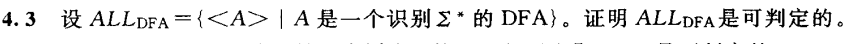
\includegraphics[width=0.8\textwidth]{chapters/imgs/hw_4_3.png}
  \caption{}
  \label{fig:hw_4_3}
\end{figure}

证明。构造判定器 $T$ 来判定
\[
    \mathrm{ALL}_{\mathrm{DFA}}
    =\{\langle A\rangle\mid A\text{ 是 DFA 且 }L(A)=\Sigma^*\}.
\]

在输入 $\langle A\rangle$ 上，其中
\[
    A=(Q,\Sigma,\delta,q_0,F),
\]
$T$ 做如下工作：

\medskip
\noindent
1. 从开始状态 $q_0$ 出发，在状态图中做一次可达性搜索，求出所有从 $q_0$ 可达的状态。

\medskip
\noindent
2. 若在这些可达状态中发现某个状态
\[
    q\notin F,
\]
则拒绝；否则接受。

\medskip
证明该算法正确。若 $T$ 接受，则每个从 $q_0$ 可达的状态都是接受态。对任意字符串 $w$，DFA $A$ 读入 $w$ 后必停在某个从 $q_0$ 可达的状态上，因此该状态接受，从而
\[
    w\in L(A).
\]
故
\[
    L(A)=\Sigma^*.
\]

反之，若 $L(A)=\Sigma^*$，则任何从 $q_0$ 可达的状态都必须是接受态；否则若某个可达状态 $q$ 不是接受态，取一条从 $q_0$ 到 $q$ 的路径所对应的字符串 $w$，则 $A$ 在输入 $w$ 上拒绝，与
\[
    L(A)=\Sigma^*
\]
矛盾。

因此 $T$ 当且仅当
\[
    \langle A\rangle\in \mathrm{ALL}_{\mathrm{DFA}}
\]
时接受。由于状态图有限，搜索必定停机，所以 $\mathrm{ALL}_{\mathrm{DFA}}$ 是可判定的。$\blacksquare$

\paragraph{解释.}
对 DFA 而言，“接受所有串”只需看一件事：从开始状态真正能到达的状态里，有没有非接受态。若有，就有某个串把机器带到那里；若没有，每个输入都会落在接受态。

\subsection*{4.4}

\begin{figure}[H]
  \centering
  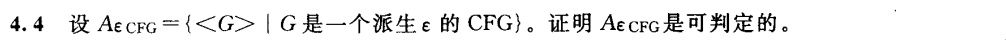
\includegraphics[width=0.8\textwidth]{chapters/imgs/hw_4_4.png}
  \caption{}
  \label{fig:hw_4_4}
\end{figure}

证明。构造判定器 $T$ 来判定
\[
    A_{\varepsilon\mathrm{CFG}}
    =\{\langle G\rangle\mid G\text{ 是 CFG 且 }\varepsilon\in L(G)\}.
\]

设
\[
    G=(V,\Sigma,R,S).
\]
我们计算所有能够生成 $\varepsilon$ 的变量。令集合 $N\subseteq V$ 初始为空，并反复执行下述标记规则：

\medskip
\noindent
若某条产生式
\[
    A\to X_1X_2\cdots X_k
\]
满足每个 $X_i$ 都属于 $N$，或者右边为空串，则把 $A$ 加入 $N$。

\medskip
由于变量个数有限，这个过程在有限步后稳定。最后若
\[
    S\in N,
\]
则接受；否则拒绝。

\medskip
下面证明正确性。先证：若某个变量 $A$ 被标记，则
\[
    A\Rightarrow^*\varepsilon.
\]
这是按标记顺序直接归纳得到的：若由规则
\[
    A\to\varepsilon
\]
被标记，则显然可推出 $\varepsilon$；若由
\[
    A\to X_1\cdots X_k
\]
被标记，且各 $X_i$ 都已能推出 $\varepsilon$，则
\[
    A\Rightarrow X_1\cdots X_k\Rightarrow^*\varepsilon.
\]

再证反向：若
\[
    A\Rightarrow^*\varepsilon,
\]
则最终 $A$ 会被标记。对这棵推出 $\varepsilon$ 的语法树做自底向上的归纳即可：叶子对应 $\varepsilon$-产生式，因此其父变量会被标记；逐层向上，整个树根 $A$ 也会被标记。

因此
\[
    S\in N
    \iff
    S\Rightarrow^*\varepsilon
    \iff
    \varepsilon\in L(G).
\]
故 $A_{\varepsilon\mathrm{CFG}}$ 是可判定的。$\blacksquare$

\paragraph{解释.}
这题的本质是求“可空变量”集合。因为一个 CFG 生成 $\varepsilon$，当且仅当开始变量是可空的；而可空性是一个有限的闭包计算问题。

\subsection*{4.6}

\begin{figure}[H]
  \centering
  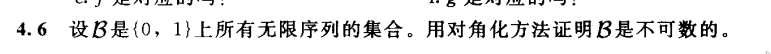
\includegraphics[width=0.8\textwidth]{chapters/imgs/hw_4_6.png}
  \caption{}
  \label{fig:hw_4_6}
\end{figure}

解答如下。

\paragraph{(a)}
$f$ 不是一一对应（one-to-one），因为
\[
    f(1)=6=f(3).
\]

\paragraph{(b)}
$f$ 不是满射（onto），因为
\[
    8,9,10
\]
都不在 $f$ 的值域中。

\paragraph{(c)}
$f$ 不是 correspondence，因为 correspondence 就是双射，而 $f$ 既不是单射也不是满射。

\paragraph{(d)}
$g$ 是一一对应的，因为
\[
    g(1)=10,\ g(2)=9,\ g(3)=8,\ g(4)=7,\ g(5)=6
\]
两两不同。

\paragraph{(e)}
$g$ 是满射的，因为它的值域恰为
\[
    \{6,7,8,9,10\}=Y.
\]

\paragraph{(f)}
$g$ 是 correspondence，因为它既是一一对应又是满射，即为双射。$\blacksquare$

\subsection*{4.10}

\begin{figure}[H]
  \centering
  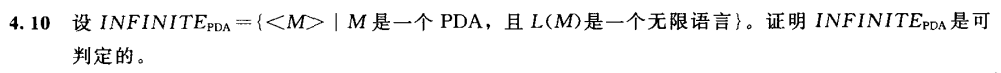
\includegraphics[width=0.8\textwidth]{chapters/imgs/hw_4_10.png}
  \caption{}
  \label{fig:hw_4_10}
\end{figure}

证明。设
\[
    P=(Q,\Sigma,\Gamma,\delta,q_0,F)
\]
是一台 DPDA。我们需要判定给定的
\[
    \langle P,q,x\rangle
\]
是否满足：从状态 $q$ 开始、以 $x$ 为当前栈顶时，机器接下来永远不读输入符号，且永远不弹出 $x$ 之下的内容。

\medskip
关键在于：在这种过程中，输入始终不被读取，因此机器的行为只取决于当前状态与栈内容；而 DPDA 又是确定的，所以从
\[
    (q,x)
\]
出发的这段 $\varepsilon$-计算是唯一的。

\medskip
定义一个有限关系
\[
    R\subseteq Q\times \Gamma\times Q,
\]
其中
\[
    (p,a,r)\in R
\]
表示：若机器处于状态 $p$，栈顶为 $a$，并且在 $a$ 之下的栈内容被冻结不动，那么机器可以仅靠 $\varepsilon$-转移，在不读取输入、也不碰到 $a$ 之下内容的前提下，最终把 $a$ 弹出并进入状态 $r$。

\medskip
关系 $R$ 可以通过有限的不动点计算得到。因为 $Q$ 和 $\Gamma$ 都有限，三元组总数有限；而某个三元组是否属于 $R$，只需检查有限多种 $\varepsilon$-转移，并递归地组合更短的“返回”情况。直观上说，这就是对 DPDA 的 $\varepsilon$-阶段做一个有限的摘要分析。

\medskip
一旦 $R$ 算出，我们便可判定 $(q,x)$ 是否为 looping situation：

\medskip
\noindent
1. 若从 $(q,x)$ 出发的唯一 $\varepsilon$-计算在某一步需要读取输入，或者在有限步后停住，则它不是 looping situation。

\medskip
\noindent
2. 若该计算能够通过 $R$ 所描述的某种返回，最终越过 $x$ 到达其下方的栈内容，则它也不是 looping situation。

\medskip
\noindent
3. 其余情形下，这段计算只能永远停留在 $x$ 及其上方，通过 $\varepsilon$-转移无限运行，因此 $(q,x)$ 正是 looping situation。

\medskip
由于上述分析完全建立在有限集合 $Q\times\Gamma\times Q$ 上，故它是一个可判定过程。于是
\[
    F=\{\langle P,q,x\rangle\mid (q,x)\text{ is a looping situation for }P\}
\]
是可判定语言。$\blacksquare$

\paragraph{解释.}
这题的难点在于栈可能无限增长，不能直接暴力模拟。但因为这里不读输入，而且 DPDA 是确定的，所以我们只需把“从某个栈顶符号出发，能否在不碰下面内容的情况下最终返回”做成有限摘要。摘要一旦算出，剩下就只是有限图上的分类：读输入、返回到底层、或永远在上面打转。

\subsection*{4.12}

\begin{figure}[H]
  \centering
  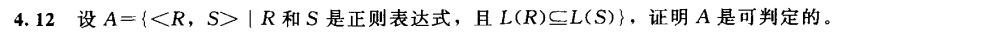
\includegraphics[width=0.8\textwidth]{chapters/imgs/hw_4_12.png}
  \caption{}
  \label{fig:hw_4_12}
\end{figure}

证明。设
\[
    A=\{\langle M_1\rangle,\langle M_2\rangle,\dots\}
\]
是一个图灵可识别语言，且其中每个 $M_i$ 都是判定器。

\medskip
若 $A$ 是有限集，则结论显然成立：因为可判定语言有无穷多个，而 $A$ 中只包含有限台判定器，因此总有某个可判定语言不由其中任何一台机器判定。

\medskip
下面设 $A$ 是无限的。由于 $A$ 图灵可识别，定理 3.13 告诉我们存在一个枚举器 $E$ 枚举 $A$ 中所有机器描述。删去重复项后，不妨设 $E$ 依次输出
\[
    \langle M_1\rangle,\langle M_2\rangle,\dots
\]

再把所有字符串按字典顺序列为
\[
    w_1,w_2,w_3,\dots
\]
定义语言
\[
    D=\{w_i\mid M_i\text{ 不接受 }w_i\}.
\]

先证 $D$ 是可判定的。给定输入 $w_i$，先模拟枚举器 $E$，直到得到第 $i$ 个不同的机器描述 $\langle M_i\rangle$。然后运行判定器 $M_i$ 于 $w_i$ 上；若 $M_i$ 接受，则拒绝，若 $M_i$ 拒绝，则接受。因为 $M_i$ 是判定器，故此过程必停机，因此 $D$ 可判定。

再证 $D$ 不被 $A$ 中任何机器判定。任取 $j\ge 1$。若 $M_j$ 判定 $D$，则看字符串 $w_j$：

\[
    w_j\in D
    \iff
    M_j\text{ 不接受 }w_j.
\]

但若 $M_j$ 判定 $D$，则
\[
    w_j\in D
    \iff
    M_j\text{ 接受 }w_j.
\]

二者矛盾。因此没有任何 $M_j$ 能判定 $D$。

故存在一个可判定语言 $D$，不被 $A$ 中出现的任何判定器所判定。$\blacksquare$

\paragraph{解释.}
这就是标准的对角化。把枚举出来的第 $i$ 台判定器和第 $i$ 个字符串配对，再在对角线上把答案反过来，于是得到的新语言和列表中第 $i$ 台机器至少在第 $i$ 个字符串上不同。

\subsection*{4.15}

\begin{figure}[H]
  \centering
  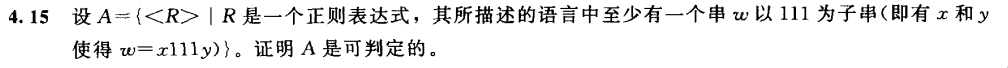
\includegraphics[width=0.8\textwidth]{chapters/imgs/hw_4_15.png}
  \caption{}
  \label{fig:hw_4_15}
\end{figure}

证明。设
\[
    C_{>}=\{w\in\{0,1\}^*\mid \#_1(w)>\#_0(w)\}.
\]
先说明 $C_{>}$ 是上下文无关语言。令
\[
    E=\{w\in\{0,1\}^*\mid \#_1(w)=\#_0(w)\}.
\]
它可由文法
\[
    S\to 0S1S\mid 1S0S\mid \varepsilon
\]
生成。再令
\[
    T\to S1S\mid S1T,
\]
则 $T$ 生成的正是 $C_{>}$，故 $C_{>}$ 是上下文无关语言。

\medskip
现在给定一台 DFA $M$。构造一个上下文无关语言
\[
    L(M)\cap C_{>}.
\]
由于上下文无关语言对与正则语言求交封闭，而 $L(M)$ 正则、$C_{>}$ 上下文无关，因此
\[
    L(M)\cap C_{>}
\]
仍是上下文无关语言。

\medskip
再由上下文无关语言的空性可判定，便可判断该交集是否为空。若
\[
    L(M)\cap C_{>}\ne\varnothing,
\]
则 $M$ 接受某个 $1$ 的个数多于 $0$ 的个数的字符串；反之则不存在这样的字符串。

因此
\[
    E=\{\langle M\rangle\mid M\text{ 是 DFA 且接受某个 }1\text{ 比 }0\text{ 多的串}\}
\]
是可判定的。$\blacksquare$

\paragraph{解释.}
题目问“DFA 是否接受某类特殊字符串”，常见套路就是和一个描述“特殊性质”的 CFL 求交，再做空性测试。这里“$1$ 比 $0$ 多”这件事本身是 CFL，所以问题就化成了一个 CFL 的空性判定。

\subsection*{4.17}

\begin{figure}[H]
  \centering
  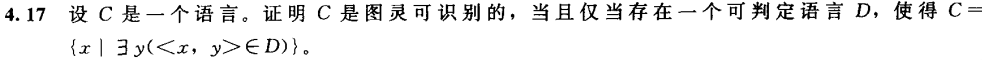
\includegraphics[width=0.8\textwidth]{chapters/imgs/hw_4_17.png}
  \caption{}
  \label{fig:hw_4_17}
\end{figure}

证明。令
\[
    C_{=}
    =\{w\in\{0,1\}^*\mid \#_0(w)=\#_1(w)\}.
\]
该语言是上下文无关的，例如由文法
\[
    S\to 0S1S\mid 1S0S\mid \varepsilon
\]
生成。

\medskip
给定一台 DFA $M$，考虑语言
\[
    L(M)\cap C_{=}.
\]
因为正则语言与上下文无关语言求交后仍是上下文无关语言，所以该交集是上下文无关语言。又由于上下文无关语言的空性可判定，我们可以测试
\[
    L(M)\cap C_{=}
\]
是否为空。

\medskip
若交集非空，则存在某个被 $M$ 接受且满足
\[
    \#_0=\#_1
\]
的字符串；若交集为空，则不存在这样的字符串。于是
\[
    \mathrm{BAL}_{\mathrm{DFA}}
    =\{\langle M\rangle\mid M\text{ 是 DFA 且接受某个 }0,1\text{ 个数相同的串}\}
\]
是可判定的。$\blacksquare$

\paragraph{解释.}
这题和 4.15 完全同型，只是把“$1$ 比 $0$ 多”换成了“$0$ 与 $1$ 个数相同”。要点仍是：先把计数条件写成一个 CFL，再与 DFA 语言求交，最后检查空性。

\subsection*{4.23}

\begin{figure}[H]
  \centering
  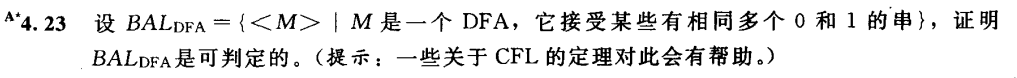
\includegraphics[width=0.8\textwidth]{chapters/imgs/hw_4_23.png}
  \caption{}
  \label{fig:hw_4_23}
\end{figure}

证明。我们给出一个可判定语言 $C$ 和一个同态 $h$，使得
\[
    h(C)=A_{\mathrm{TM}}.
\]
这将说明可判定语言类在同态下并不封闭，因为
\[
    A_{\mathrm{TM}}
\]
是不可判定的。

\medskip
设
\[
    C=\{\overline{\langle M,w\rangle}\#c\mid c\text{ 是 }M\text{ 在 }w\text{ 上的一个接受计算历史}\}.
\]
这里 $\overline{\langle M,w\rangle}$ 表示把编码 $\langle M,w\rangle$ 中的每个符号都换成一个“带横线的副本”，从而使它们和计算历史 $c$ 所使用的普通字母表互不混淆。

\medskip
先证 $C$ 可判定。给定输入
\[
    \overline{\langle M,w\rangle}\#c,
\]
我们只需检查以下有限条件：

\medskip
\noindent
1. $c$ 的第一项是否是 $M$ 在输入 $w$ 上的初始配置；

\medskip
\noindent
2. $c$ 的最后一项是否为接受配置；

\medskip
\noindent
3. $c$ 中每一对相邻配置是否满足 $M$ 的转移规则。

\medskip
这些检查都是机械可做的，因此 $C$ 是可判定语言。

\medskip
现在定义同态 $h$ 如下：

\medskip
\noindent
对每个带横线的符号 $\overline a$，令
\[
    h(\overline a)=a;
\]

\medskip
\noindent
对分隔符 $\#$ 以及计算历史部分所使用的普通符号，令
\[
    h(b)=\varepsilon.
\]

\medskip
于是对任意字符串
\[
    \overline{\langle M,w\rangle}\#c\in C,
\]
都有
\[
    h(\overline{\langle M,w\rangle}\#c)=\langle M,w\rangle.
\]
并且
\[
    \langle M,w\rangle\in h(C)
    \iff
    \exists c\ \big(c\text{ 是 }M\text{ 在 }w\text{ 上的接受计算历史}\big)
    \iff
    \langle M,w\rangle\in A_{\mathrm{TM}}.
\]

因此
\[
    h(C)=A_{\mathrm{TM}}.
\]
由于 $C$ 可判定而 $A_{\mathrm{TM}}$ 不可判定，可判定语言类在同态运算下不封闭。$\blacksquare$

\paragraph{解释.}
这里的技巧是把“不可判定性”藏在被擦掉的那一部分里。原语言 $C$ 本身只是在验证一个给定的接受计算历史，因此是可判定的；但一旦用同态把计算历史抹掉，只留下 $\langle M,w\rangle$，就恢复成了 $A_{\mathrm{TM}}$。

\subsection*{4.27}

\begin{figure}[H]
  \centering
  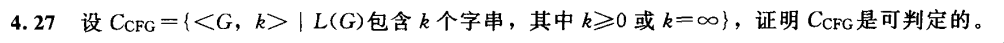
\includegraphics[width=0.8\textwidth]{chapters/imgs/hw_4_27.png}
  \caption{}
  \label{fig:hw_4_27}
\end{figure}

证明。给定一个 CFG $G$，我们要判定是否有
\[
    1^*\subseteq L(G).
\]

\medskip
先构造一个正则语言
\[
    R=1^*.
\]
由上下文无关语言对与正则语言求交封闭，可有效构造出一个 CFG $G'$，使得
\[
    L(G')=L(G)\cap 1^*.
\]

\medskip
于是 $L(G')$ 是一个一元字母表
\[
    \{1\}
\]
上的上下文无关语言。由经典定理可知：每个一元上下文无关语言都是正则语言，而且从其 CFG 可以有效构造出等价的 DFA。于是可有效得到某个 DFA $A$，满足
\[
    L(A)=L(G').
\]

\medskip
现在只需判断
\[
    L(A)=1^*
\]
是否成立。由于 DFA 的全语言问题 $\mathrm{ALL}_{\mathrm{DFA}}$ 是可判定的，等价地，也可判定两个 DFA 是否识别同一语言，因此这个测试是可判定的。

\medskip
最后注意到
\[
    1^*\subseteq L(G)
    \iff
    L(G)\cap 1^*=1^*
    \iff
    L(G')=1^*.
\]
因此
\[
    \{\langle G\rangle\mid G\text{ 是 }\{0,1\}\text{ 上的 CFG 且 }1^*\subseteq L(G)\}
\]
是可判定语言。$\blacksquare$

\paragraph{解释.}
题目的难点在于：一般 CFG 的“全包含”问题不可判定，但这里只要求覆盖
\[
    1^*
\]
这一条一元正则子语言。与 $1^*$ 相交后，问题落到一元 CFL 上，而一元 CFL 实际上就是正则语言，于是又回到了 DFA 可判定的范围。

\clearpage
